% Diagram arsitektur ringkas. Versi lengkap: arsitektur_detail.tex
% Kompilasi (dari folder ini): pdflatex arsitektur.tex && pdftoppm -png -r 300 -singlefile arsitektur.pdf arsitektur
\documentclass[border=6pt]{standalone}
\usepackage{mathptmx}
\usepackage{tikz}
\usetikzlibrary{arrows.meta, shadows, calc}

\definecolor{ink}{HTML}{3A3936}
\definecolor{muted}{HTML}{8A8984}
\definecolor{dataF}{HTML}{F0EFEC}
\definecolor{modelE}{HTML}{2A78D6}\definecolor{modelF}{HTML}{DCE9F9}
\definecolor{augE}{HTML}{EB6834}\definecolor{augF}{HTML}{FDE3D6}
\definecolor{opE}{HTML}{6250D6}\definecolor{opF}{HTML}{EBE9FB}
\definecolor{lossE}{HTML}{1BAF7A}\definecolor{lossF}{HTML}{D9F3E9}

\tikzset{
  every node/.style={font=\small, text=ink, align=center},
  base/.style={rectangle, rounded corners=3pt, minimum height=10mm, inner sep=3pt, line width=0.8pt},
  data/.style={base, fill=dataF, draw=muted, text width=22mm},
  model/.style={base, fill=modelF, draw=modelE, text width=17mm},
  aug/.style={base, fill=augF, draw=augE, line width=1.2pt, text width=24mm},
  outp/.style={base, fill=opF, draw=opE, text width=19mm},
  loss/.style={base, fill=lossF, draw=lossE, text width=28mm},
  tensor/.style={rectangle, fill=white, draw=modelE, line width=0.8pt, minimum width=6mm, minimum height=8.5mm,
                 double copy shadow={shadow xshift=1.6pt, shadow yshift=1.6pt, draw=modelE, fill=white}},
  flow/.style={-{Stealth[length=2.3mm]}, line width=0.8pt, draw=ink, rounded corners=4pt},
}

\begin{document}
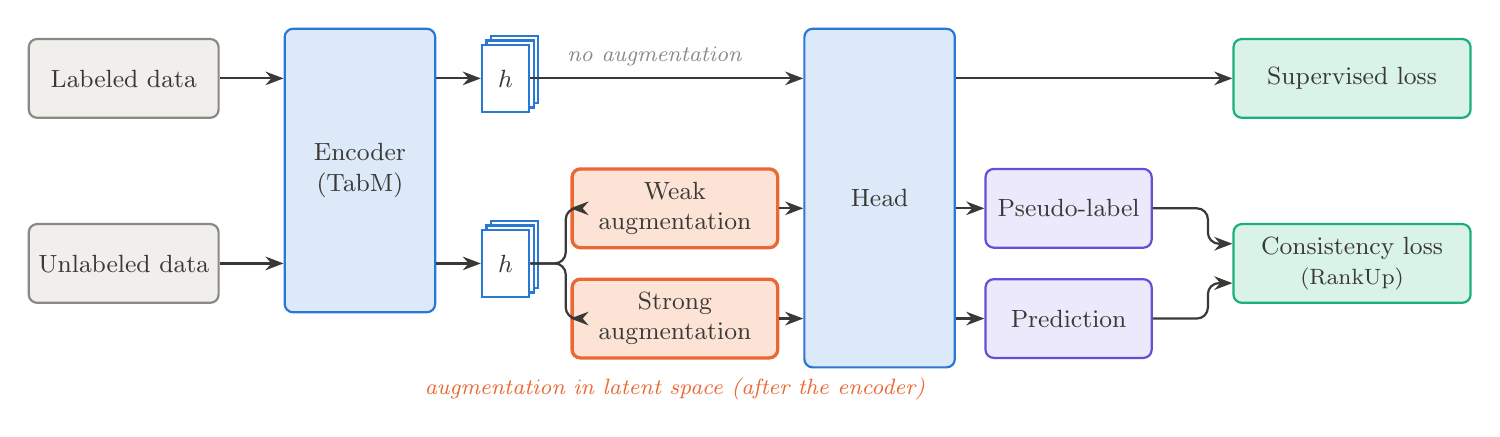
\begin{tikzpicture}
\def\yL{0} \def\yU{-2.35} \def\yW{-1.65} \def\yS{-3.05}

\node[data] (xl) at (0,\yL) {Labeled data};
\node[data] (xu) at (0,\yU) {Unlabeled data};

\node[model, minimum height=36mm] (enc) at (3.0,-1.17) {Encoder\\(TabM)};
\node[tensor] (hl) at (4.85,\yL) {$h$};
\node[tensor] (hu) at (4.85,\yU) {$h$};

\node[aug] (aw) at (7.0,\yW) {Weak\\augmentation};
\node[aug] (as) at (7.0,\yS) {Strong\\augmentation};

\node[model, minimum height=43mm] (head) at (9.6,-1.52) {Head};

\node[outp] (pl) at (12.0,\yW) {Pseudo-label};
\node[outp] (pr) at (12.0,\yS) {Prediction};
\node[loss] (lc) at (15.6,\yU) {Consistency loss\\{\footnotesize (RankUp)}};
\node[loss] (ls) at (15.6,\yL) {Supervised loss};

\draw[flow] (xl) -- (xl -| enc.west);
\draw[flow] (xu) -- (xu -| enc.west);
\draw[flow] (enc.east |- hl) -- (hl);
\draw[flow] (enc.east |- hu) -- (hu);
\draw[flow] (hl) -- (hl -| head.west);
\draw[flow] (hu.east) -- ++(0.45,0) |- (aw.west);
\draw[flow] (hu.east) -- ++(0.45,0) |- (as.west);
\draw[flow] (aw) -- (aw -| head.west);
\draw[flow] (as) -- (as -| head.west);
\draw[flow] (head.east |- ls) -- (ls);
\draw[flow] (head.east |- pl) -- (pl);
\draw[flow] (head.east |- pr) -- (pr);
\draw[flow] (pl.east) -- ++(0.7,0) |- ([yshift=2.5mm]lc.west);
\draw[flow] (pr.east) -- ++(0.7,0) |- ([yshift=-2.5mm]lc.west);

\node[font=\footnotesize\itshape, text=muted, above=1pt] at ($(hl)!0.5!(hl -| head.west)$) {no augmentation};
\node[font=\footnotesize\itshape, text=augE, below=3pt] at (as.south) {augmentation in latent space (after the encoder)};
\end{tikzpicture}
\end{document}
